% \vskip -1em
\section{\textbf{Stages:} early-stage plasticity loss becomes irrecoverable}
\label{Sec: Stages}
\vskip -0.5em

In this section, we elucidate the differential attributes of plasticity loss throughout various training stages.
Upon confirming that the critic's plasticity loss is central to hampering training efficiency, a closer review of the results in Figure~\ref{Fig:FAU} underscores that DA's predominant contribution is to effectively recover the critic's plasticity during initial phases.
This naturally raises two questions:
\textcolor{myorange}{$\bullet$}~After recovering the critic's plasticity to an adequate level in the early stage, will ceasing interventions to maintain plasticity detrimentally affect training?
\textcolor{myblue}{$\bullet$}~If interventions aren't applied early to recover the critic's plasticity, is it still feasible to enhance training performance later through such measures?
To address these two questions, we conduct a comparative experiment by turning on or turning off DA at certain training steps and obtain the following findings:
% The findings in Figure~\ref{Fig:Turn DA} provide a compelling response:
\textcolor{myorange}{$\bullet$ Turning off DA} after the critic's plasticity has been recovered does not affect training efficiency.
This suggests that it is not necessary to employ specific interventions to maintain plasticity in the later stages of training.
\textcolor{myblue}{$\bullet$ Turning on DA} when plasticity has already been significantly lost and without timely intervention in the early stages cannot revive the agent's training performance.
This observation underscores the vital importance of maintaining plasticity in the early stages; otherwise, the loss becomes irrecoverable.

\begin{figure}[ht]
  \centering
  \vspace{-0.5\baselineskip}
  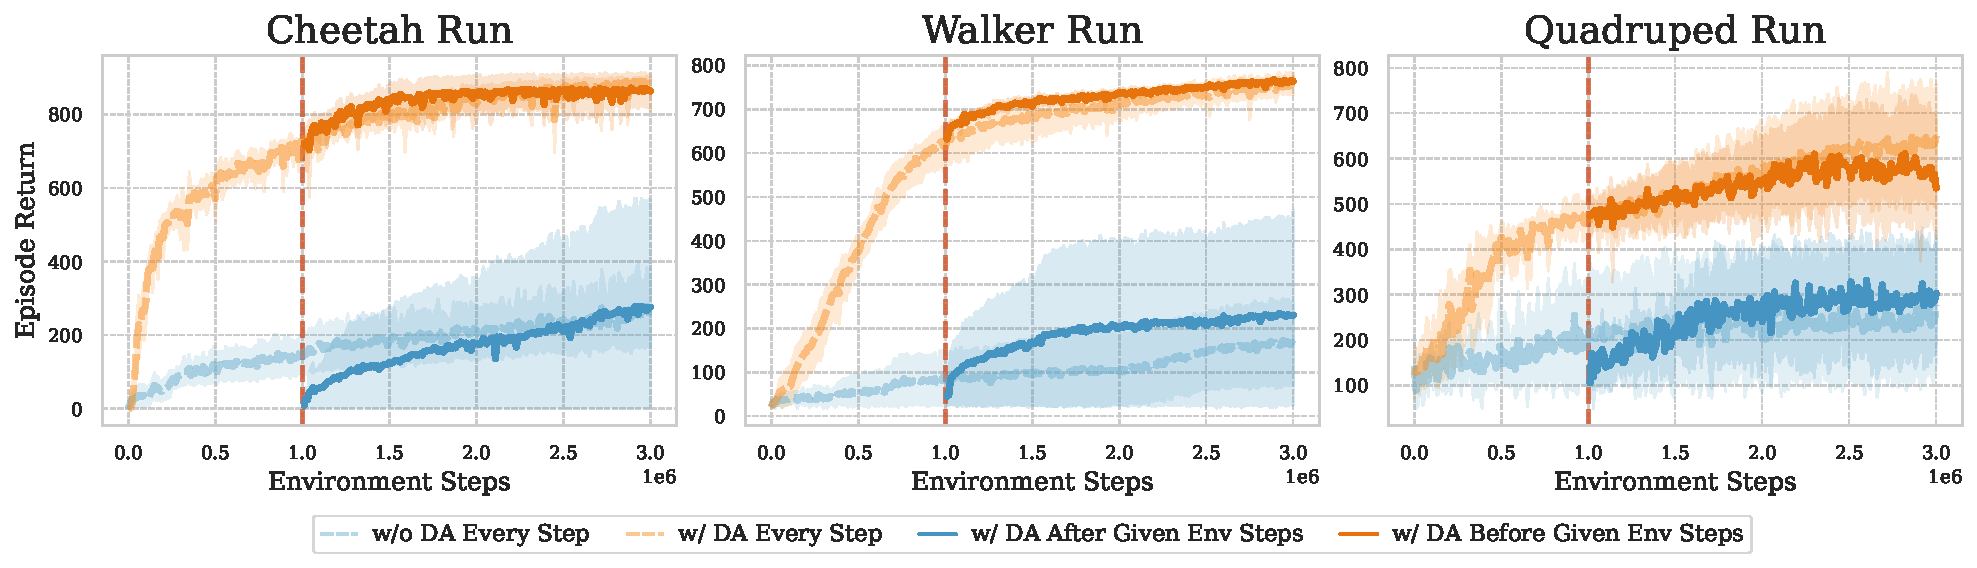
\includegraphics[width=\textwidth]{Figures/3Stages/recover_1M.pdf} 
  \vspace{-1.5\baselineskip}
  \caption{Training curves for various DA application modes. The red dashed line shows when DA is \textcolor{myblue}{turned on} or \textcolor{myorange}{turned off}. Additional comparative results can be found in \Appendix~\ref{Appendix: Turning DA}.}
  \label{Fig:Turn DA}
\end{figure}

\vspace{-0.5\baselineskip}

We attribute these differences across stages to the nature of online RL to learn from scratch in a bootstrapped fashion.
During the initial phases of training, bootstrapped target derived from low-quality and limited-quantity experiences exhibits high non-stationarity and deviates significantly from the actual state-action values~\citep{A-LIX}.
The severe non-stationarity of targets induces a rapid decline in the critic's plasticity~\citep{Enhancing_Generalization_Plasticity, Regulating_Overfitting}, consistent with the findings in Figure~\ref{Fig:FAU}.
Having lost the ability to learn from newly collected data, the critic will perpetually fail to capture the dynamics of the environment, preventing the agent from acquiring an effective policy.
This leads to \textbf{\textit{catastrophic plasticity loss}} in the early stages.
Conversely, although the critic's plasticity experiences a gradual decline after recovery, this can be viewed as a process of progressively approximating the optimal value function for the current task.
For single-task VRL that doesn't require the agent to retain continuous learning capabilities, this is termed as a \textbf{\textit{benign plasticity loss}}.
Differences across stages offer a new perspective to address VRL's plasticity loss challenges.

% Early Stage is The plasticity-recovery stage

% plasticity is recoverable and easy to loss

% late stage: irrecoverable